\documentclass[tikz,border=10pt]{standalone}
\usepackage{tikz}
\usetikzlibrary{positioning, shapes.geometric, arrows.meta, fit, calc, matrix}

\begin{document}
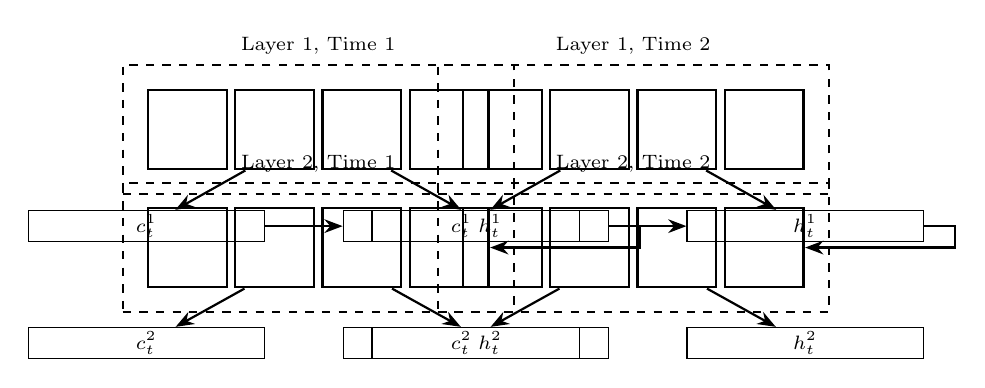
\begin{tikzpicture}[
    cell/.style={rectangle, draw, minimum size=10mm, thick},
    arrow/.style={-Stealth, thick},
    every node/.style={font=\scriptsize},
    vector/.style={rectangle, draw, minimum width=30mm, minimum height=4mm, inner sep=0pt},
    layerbox/.style={rectangle, draw, dashed, thick, inner sep=3mm}
]

% Parameters for ease of adjustments
\newcommand{\NumCells}{4}
\newcommand{\NumLayers}{2}
\newcommand{\Timesteps}{2}
\newcommand{\LayerSep}{1.5}
\newcommand{\CellSep}{0.8}
\newcommand{\TimeSep}{4}
\newcommand{\VectorSep}{0.4}

% Define matrix positions
\foreach \l in {1,...,\NumLayers}{
    \foreach \t in {1,...,\Timesteps}{
        \matrix[matrix of nodes, nodes in empty cells, column sep=\CellSep mm, row sep=1mm, inner sep=0pt, ampersand replacement=\&] at (\t*\TimeSep,-\l*\LayerSep) (matrix-\l-\t) {
            |[cell]| \& |[cell]| \& |[cell]| \& |[cell]| \\
        };
        
        % Draw layer box around cells
        \node[layerbox, fit=(matrix-\l-\t)] (layerbox-\l-\t) {};
        \node[above=0pt of layerbox-\l-\t.north] {Layer \l, Time \t};
    }
}

% Draw c_t and h_t vectors
\foreach \t in {1,...,\Timesteps}{
    \foreach \l [evaluate=\l as \yshift using {(\l-1)*\VectorSep}] in {1,...,\NumLayers}{
        \node[vector, below=5mm of matrix-\l-\t.south west, yshift=\yshift] (c-\l-\t) {$c_t^\l$};
        \node[vector, below=5mm of matrix-\l-\t.south east, yshift=\yshift] (h-\l-\t) {$h_t^\l$};
        \draw[arrow] (matrix-\l-\t) -- (c-\l-\t);
        \draw[arrow] (matrix-\l-\t) -- (h-\l-\t);
    }
}

% Draw arrows representing flow between timesteps for the last layer
\foreach \t [evaluate=\t as \nextt using int(\t+1)] in {1,...,\NumLayers}{
    \ifnum\t<\Timesteps\relax
        \draw[arrow] (h-\t-\t) -- (h-\t-\nextt.west);
        \draw[arrow] (c-\t-\t) -- (c-\t-\nextt.west);
    \fi
}

% Draw arrows representing flow between layers within a timestep
\foreach \t in {1,...,\Timesteps}{
    \foreach \l [evaluate=\l as \nextl using int(\l+1)] in {1,...,\NumLayers}{
        \ifnum\l<\NumLayers\relax
            \draw[arrow] (h-\l-\t.east) -- ([xshift=\VectorSep cm]h-\l-\t.east) |- (matrix-\nextl-\t);
        \fi
    }
}

\end{tikzpicture}
\end{document}
